\documentclass[]{article}

% Packages
\usepackage{amsmath} % math stuff
%\usepackage[dvipsnames]{xcolor}  % for coloring
\usepackage{tensor}  % tensors, but also for stuff like superscript on the left
\usepackage{enumitem} % for enumerating alphabetically
\usepackage{tabto}		% for tabbing to a certain length
\usepackage{scrextend} % for local margins
\usepackage{titling}	% for subtitle custom command
\usepackage[svgnames, table]{xcolor} % avoid the option clash for hyperref command  + TABLE REP
\usepackage[colorlinks=true, linkcolor=Blue, urlcolor=Blue]{hyperref} % for hyperref command 
\usepackage{pgfplots} % plots


%tables for list representation
\usepackage{arydshln, collcell}
\newcolumntype{C}{>{\collectcell\mathsf}c<{\endcollectcell}}


%Repeat command
\usepackage{expl3}
\ExplSyntaxOn
\cs_new_eq:NN \Repeat \prg_replicate:nn
\ExplSyntaxOff

% Algorithms
\usepackage{algorithm}
\usepackage{algorithmicx}
\usepackage[noend]{algpseudocode}
\newcommand{\Get}{\State \textbf{get}~}
\newcommand{\Set}{\State \textbf{set}~}
\newcommand{\Print}{\State \textbf{print}~}
\newcommand{\Getx}[1]{\Statex \algindent{#1} \textbf{get}~}		% x denotes non-numbered lines
\newcommand{\Setx}[1]{\Statex \algindent{#1} \textbf{set}~}	% enter the number of lines to indent
\newcommand{\Printx}[1]{\Statex \algindent{#1} \textbf{print}~}
\newcommand{\Stop}{\State \textbf{stop}~}
\newcommand{\algindent}[1]{\Repeat{#1}{\hskip\algorithmicindent}}
\algdef{SE}[DOWHILE]{Do}{doWhile}{\algorithmicdo}[1]{\algorithmicwhile\ (#1)}


% stop indentation
\setlength{\parindent}{0pt}

% custom subtitle command
\newcommand{\subtitle}[1]{
	\posttitle{
		\par\end{center}
	\begin{center}\large#1\end{center}
	\vskip0.5em}
}


% Fixes weird backwards quote thing
\usepackage [english]{babel}
\usepackage [autostyle, english = american]{csquotes}
\MakeOuterQuote{"}

% fix upside down exclaimation points for less thans or greater thans
\usepackage[T1]{fontenc}


% Title
\title{CS 201 Notes}
\subtitle{Introduction to Computer Science}
\author{Jaeden Bardati}
\date{\textit{Last modified \today}}

\setcounter{section}{-1}	% 0-indexes the section

\begin{document}

\maketitle
\bigbreak

% Course Video 0
\section{Course Overview\\ {\large \normalfont September 10, 2021}}
\bigbreak

\subsection{What is Computer Science?}
\bigbreak

Computer science is the study of \textbf{algorithms}.\\\\
An \textbf{algorithm} is an effective method for solving a problem, expressed as a finite sequence of steps.\\\\
The development of algorithms works in this recurring order:
\begin{itemize}
	\item \textbf{Design}
	\item \textbf{Analysis}
	\item \textbf{Implement}
	\item \textbf{Experiment}\smallskip
\end{itemize}

\noindent In the \textbf{design} phase, we design an algorithm using pseudo-code. In the \textbf{analysis} phase, we need to analyze the correctness and the efficiency. That is to say, we make sure that our algorithm will work and completes in a reasonable amount of time. During the \textbf{implementation}, the algorithm is written in code on a computer. Finally, the algorithm is run and debugged in the \textbf{experiment} phase. This process repeats.


\section{Introduction to Algorithms}
\bigbreak

% Course Video 1
\subsection{Design\\ {\normalfont September 11, 2021}}
\bigbreak

An algorithm is a step by step procedure to solve a problem. For example, 
\begin{itemize}
	\item Step 1: Do something
	\item Step 2: Do something
	\item ...
	\item Step n: Do something\smallskip
\end{itemize}

\noindent There are three basic types of steps. Note that there is a fourth (recursion), but it is not covered in this course. 
\subsubsection{Sequential Steps}
\bigbreak
	\textbf{Do a single task}.\\\\
	\textit{For example:} Let $x$ be a variable. A sequential step could be to add 1 to $x$.
\subsubsection{Conditional Steps}
\bigbreak
	\textbf{Ask a question} that supports only \textbf{logic answers} (true or false answer). \\\\
	\textit{For example:} Let $x$ be a variable. A conditional step could be to ask if $x > 0$. If so, add 1 to $x$; otherwise, subtract 1 from $x$.
\subsubsection{Iterative Steps (loops)}
\bigbreak
	\textbf{Repeat a task} until a certain condition is satisfied. This step links the sequential step to the conditional steps.\\\\
	\textit{For example:} If you have a recipe that you need to add water until its dry. An iterative step would be one where you add $\frac{1}{2}$ cup to mixture while mixture is dry.


% Course Video 2 and 3
\subsection{Case Study: Addition Algorithm\\ {\normalfont September 11, 2021}}
\bigbreak

Let's say we want to add 472 to 593. We would to it like so:\\\\
\begin{tabular}{cccc}
	& \tiny 1 & \tiny & \tiny \\
	& 4 & 7 & 2 \\
	+ & 5  & 9 & 3 \\
	\hline
	1 & 0 & 6 & 5 \\
\end{tabular}
\medbreak
\noindent If you know how to add these numbers, you know how to do it for any numbers. Why? Because we used a sequence of steps to solve it: We used an algorithm. What is this algorithm?\\

\noindent We know that we can break down the work for each of the digits. It is an iterative statement for each digit. What is the work we need to do at each iteration?\\

\noindent First, we add the digits plus the carry in (starts at 0). This is a \textbf{sequential step}. Then, we ask if it is greater than 9. If so, we set the resulting digit as the addition subtracted by 10 and set the carry out (which is te carry in for the next step) to 1; otherwise, we simply set the resulting digit as the addition and set the carry out to be 0. This is a \textbf{conditional step}. Then we repeat this process until we have no more digits to add. This is an \textbf{iterative step}.\\

\noindent Now, we need to conceptualize this. Let's let $m \geq 1$ be the number of digits. Let us define $a_i$ (first number digits), $b_i$ (second number digits) and $c_i$ (resulting number digits) as follows:

\begin{tabular}{ccccc}
	& \tiny & \tiny & \tiny & \tiny \\
	& $a_{m-1}$ & ... & $a_{1}$ & $a_{0}$ \\
	+ & $b_{m-1}$ & ... & $b_{1}$ & $b_{0}$ \\
	\hline
	$c_{m}$ & $c_{m-1}$ & ... & $c_{1}$ & $c_{0}$ \\\smallskip
\end{tabular}

\noindent Let's write the steps of our algorithm:

\begin{algorithm}
	\caption{\\Addition Algorithm}
	\begin{algorithmic}[1]
		\Get $m$ (provided by user)
		\Get $a_{m-1}$, ...  $a_{1}$, $a_{0}$ and $b_{m-1}$, ...  $b_{1}$, $b_{0}$ (provided by user)
		\Set $i = 0$ (digit index) and carry = 0
		\While{($i \leq m - 1$)}
			\Set $c_i = a_i + b_i$ + carry
			\If{($c_i \geq 10$)}
				\Set $c_i = c_i - 10$
				\Set carry = 1
			\Else
				\Set carry = 0
			\EndIf
			\Set $i = i + 1$
		\EndWhile
		\Set $c_m$ = carry
		\Print $c_{m-1}$, ...  $c_{1}$, $c_{0}$
		\Stop
	\end{algorithmic}
\end{algorithm}

\noindent This can be programmed now using a programming language.\\

\noindent If you want to test your algorithm, you can perform a \textbf{trace}. A trace is when you go through the algorithm yourself step by step for a test case.


% Course Video 4, 5, 6 and 7
\subsection{Pseudocode\\ {\normalfont September 11, 2021}}
\bigbreak

Pseudocode is:

\begin{itemize}
	\item Simplified
	\item A tradeoff between natural and programming languages
	\item Not unique\smallskip
\end{itemize}

\noindent We will now look into the types of statements and the syntax we will use.

\subsubsection{Sequential statements}
\bigbreak
\begin{itemize}
	\item \textbf{Input}: Get "variable". E.g. Get $m$, Get radius
	\item \textbf{Computation}: Set variable = expression. E.g. Set area = $\pi \times$ radius$^2$
	\item \textbf{Output}: Print "variable". E.g. Print area.\smallskip
\end{itemize}

\begin{algorithm}
	\caption{\\Calculates the average of three numbers.}
	\begin{algorithmic}[1]
		\Get $x, y, z$
		\Set average = $\frac{x + y + z}{3}$
		\Print average
		\Stop
	\end{algorithmic}
\end{algorithm}

\subsubsection{Conditional statements}
\bigbreak
\begin{itemize}
	\item If (condition) Then\\
				\tabto{0.5cm}operation T$_1$\\
				\tabto{0.5cm}operation T$_2$\\ 
				\tabto{0.5cm}...\\
				\tabto{0.5cm}operation T$_\mathrm{m}$\\
			Else\\
				\tabto{0.5cm}operation F$_1$\\
				\tabto{0.5cm}operation F$_2$\\ 
				\tabto{0.5cm}...\\
				\tabto{0.5cm}operation F$_\mathrm{n}$\smallskip
\end{itemize}

\begin{algorithm}
	\caption{\\Print average of three number if the first number is larger than 0, otherwise print an error message.}
	\begin{algorithmic}[1]
		\Get $x, y, z$
		\If{($x \geq 0$)}
			\Set average = $\frac{x + y + z}{3}$
			\Print average
		\Else	
			\Print "Bad Data"
		\EndIf
		\Stop
	\end{algorithmic}
\end{algorithm}

\noindent When a conditional statements within a conditional statement it is called a \textbf{nested} conditional statements (or nested ifs). This also applies to nested iterative statements (or nested loops).


\subsubsection{Iterative statements}
\bigbreak
\begin{itemize}
	\item While (condition) Do step $i$ to step $j$ \setlength{\itemindent}{0.5cm}
		\item Step $i$: operation
		\item Step $i + 1$: operation
		\item ...
		\item Step $j$: operation
	\setlength{\itemindent}{0cm}\item Stop\smallskip
\end{itemize}

\noindent There are some considerations that you have to be careful of when writing a while loop:\\
\begin{addmargin}[2em]{0em}
	If the condition is initially false, the loop will not execute at all.\\\\
	If the condition is initially true, the loop is iterated until the condition is false. This means that \textit{at least one step should change the condition at some point}. If this is forgotten, the loop will run forever (called an \textbf{infinite loop})! This is considered a \textbf{fatal error}.\\
\end{addmargin}


\begin{algorithm}
	\caption{\\Compute and print the square of the first 100 integers.}
	\begin{algorithmic}[1]
		\Set index=1
		\While{(index $\leq$ 100)}
			\Set square = index * index
			\Print square
			\Set index = index + 1
		\EndWhile
		\Stop
	\end{algorithmic}
\end{algorithm}


% Course video 8
\subsubsection{The Do-While\\ {\normalfont September 23, 2021}}
\bigbreak

The do-while is similar to the while-do, but you check the condition after the do section.

\begin{itemize}
	\item Do \setlength{\itemindent}{0.5cm}
	\item Step $i$: operation
	\item Step $i + 1$: operation
	\item ...
	\item Step $j$: operation
	\setlength{\itemindent}{0cm}\item While (condition)\smallskip
\end{itemize}

This will always execute at least once. It will only execute once if the condition is false, and multiple if it is true. For example,

\begin{algorithm}
	\caption{\\Read a var $x$, print $\sqrt{x}$ and repeat the process as long as requested by user.}
	\begin{algorithmic}[1]
		\Get $x$
		\Do
			\Get $x$
			\If{($x \geq 0 $)}
				\Set root = $\sqrt{x}$
				\Print root
			\Else
				\Print "Bad data"
			\EndIf
			\Print "Do you want to continue? Y/N"
			\Get continue
		\doWhile{continue == 'Y'}
		\Stop
	\end{algorithmic}
\end{algorithm}


% Course video 9 and 10
\subsection{The Sequential Search Algorithm\\ {\normalfont September 24, 2021}} \label{sequentialsearchalgorithm}
\bigbreak

Given a dataset of a given size $N$ and given a target, is the target in the dataset?\\

For example, if the dataset is the list [13, 4, 5, -20, 45, 112] with $N = 6$. Is the target 45 in the dataset? Yes. Is the target 130 in the dataset? No. \\

To solve for much larger values of N, we can search sequentially through the list until we reach the target (the target is in the list), or the end of the list (the target is not in the list).\\

Let us assume we have a list of size $N$ whose elements are $L_1$, $L_2$, ..., $L_N$ and a target element called Target.

\begin{algorithm}
	\caption{\\Sequential Search Algorithm}
	\begin{algorithmic}[1]
		\Get $L_1$, $L_2$, ..., $L_N$, $N$, Target
		\Set Found = No
		\Set $i$ = 1
		\While{Found = No AND $i$ <= $N$}
			\If{($L_i$ == Target)}
				\Set Found = Yes
			\Else
				\Set $i$ = $i$ + 1
			\EndIf
		\EndWhile
		\If{Found = Yes}
			\Print "Target in list."
		\Else
			\Print "Target not in list."
		\EndIf
		\Stop
	\end{algorithmic}
\end{algorithm}

% Course video 12 and 13 (what happened to 11?... no clue, probably best not to ask)
\subsection{Find Largest\\ {\normalfont September 25, 2021}}
\bigbreak

Given a list of $N$ elements, what is the largest element in the list?\\

For example, if the list is [19, 41, 12, 63, 22] with $N = 5$. Each element has an index (1, 2, 3, 4, and 5, respectively). The largest element is 63.\\

To solve, we can store a value for the largest value starting with the first number and then iterate through each other element of the list and update the largest number to the current element if it is larger than the stored value for the largest element.\\

Let us assume we have a list of size $N$ whose elements are $L_1$, $L_2$, ..., $L_N$.

\begin{algorithm}
	\caption{\\Find Largest}
	\begin{algorithmic}[1]
		\Get $N$, $L_1$, $L_2$, ..., $L_N$
		\Set $i$ = 2
		\Set largest = $L_1$
		\algstore{findlargest}
	\end{algorithmic}
\end{algorithm}
\begin{algorithm}
	\begin{algorithmic}[1]
		\algrestore{findlargest}
		\Set index = 1
		\While{$i$ <= $N$}
			\If{($L_i$ > largest)}
				\Set largest = $L_i$
				\Set index = $i$
			\EndIf
			\Set $i$ = $i$ + 1
		\EndWhile
		\Print largest
		\Stop
	\end{algorithmic}
\end{algorithm}


% Course video 14
\subsection{The Swap Algorithm\\ {\normalfont September 25, 2021}}
\bigbreak

Assume we have two variables $x$ and $y$ and want to swap them. Let us say, $x = 5$ and $y = 5$. After the swap we want $x = 3$ and $y = 5$.\\

To do this, we could try simply setting $x = y$ and then $y = x$. Doing this would simply make $x = y = 3$. Thus, we need a temporary variable to store the value of $x$ in during the swap.

\begin{algorithm}
	\caption{\\Swap(x, y)}
	\begin{algorithmic}[1]
		\Require $x$, $y$
		\Set temp = $y$
		\Set $y$ = $x$
		\Set $x$ = temp
	\end{algorithmic}
\end{algorithm}


% Course video 15
\subsection{The Gauss Sum\\ {\normalfont September 25, 2021}}
\bigbreak

Gauss was a mathematician who came up with a method to do the following. Let's assume $n > 1$. We want to find the result of the sum = 1 + 2 + 3 + ... + $n$. For $n = 5$, then sum = 1 + 2 + 3 + 4 + 5 = 15.

\begin{algorithm}
	\caption{\\Gauss Sum}
	\begin{algorithmic}[1]
		\Get $n$
		\Set sum = 0
		\Set $i$ = 1
		\While{($i \leq n$)}
			\Set sum = sum + $i$
			\Set $i$ = $i + 1$
		\EndWhile
		\Print sum
		\Stop
	\end{algorithmic}
\end{algorithm}


Gauss, however, noticed that sum = $\frac{n(n+1)}{2}$. For $n = 5$, sum = $\frac{5(5+1)}{2} = 15$. This makes the algorithm much faster.


% Course video 16
\subsection{Algorithms Efficiency (Complexity)}
\bigbreak

An algorithm is \textbf{efficient} if it uses the smallest number of steps to solve the problem. What we are really interested in is how well the algorithm \textit{scales} with large datasets. \\

For example, assume the size of the data is $n$ and two correct algorithms. \\ 

Algorithm 1 is 20 steps. \par 
Algorithm 2 is 15 steps. \\

Which is the best algorithm? You might think that the best algorithm is the one that uses 15 steps. You are probably wrong.\\

Why? When we refer to "steps" in the algorithmic efficiency definition, we really mean the number of CPU operations not the number of steps written in the algorithm. We could have a loop that causes the algorithm to run much longer than one without a loop. So the number of steps in the written algorithm is not a good measure of efficiency.\\

Assume we have some arbitrary algorithm for a dataset of size $n$ with a loop and some sequential steps. 

\begin{itemize}
	\item $n$ small ---------------------------------> very large $n$
	\item Sequential statement ---------------> Cost is the same
	\item Conditional statement --------------> Cost is the same
	\item Iterative statement ------------------> Cost increases
\end{itemize}

Thus, \textbf{efficiency} is related to the loops in the algorithm. When we say \textbf{efficiency analysis}, we really mean \textit{loop analysis}.


% Course video 17 and 18
\subsubsection{Case Study: Sequential Search\\ {\normalfont October 5, 2021}}
\bigbreak

We will analyze the efficiency of the \hyperref[sequentialsearchalgorithm]{Sequential Search Algorithm}. \\

\textbf{Best case scenario:} The algorithm will stop immediately. The number of iterations is 1.\\

\textbf{Worst case scenario:} The algorithm will go through all elements before stopping. The number of iterations is $n$.\\

\textbf{Average case scenario:} The target has an equal likelihood to be in any location (1, 2, 3, 4, ..., n). The average is therefore $\frac{1+2+3+4+...+n}{n}$. This is a Gauss sum which equals $\frac{(n+1)n}{2n} = \frac{n+1}{2} = \frac{n}{2} + \frac{1}{2}$. Thus, the average case scenario has a number of iterations $\frac{n+1}{2}$.\\


We will now do a \textbf{time analysis.}\\

Assume that the time required for 1 iteration is $C$ (depending on the computer).\\

\textbf{Worst case scenario:} $t_{\mathrm{worst}} = C n$\\

\textbf{Average case scenario:} $t_{\mathrm{avg}} = C (\frac{n}{2} + \frac{1}{2}) = \frac{1}{2}Cn + \frac{1}{2}C 
\approx \frac{1}{2}Cn$ for large $n$.\\


We can interpret these results in the following graph.\bigbreak

\begin{center}
	\begin{tikzpicture}
		\begin{axis}[ 
			xlabel=$n$,
			ylabel={time},
			xmin=0,
			ymin=0,
			xmax=100,
			ymax=100,
			yticklabels={,,},
			xticklabels={,,},
			tick style={draw=none}
			] 
			\addplot[domain=0:100, samples=10, color=blue]{3*x/2};
			\addlegendentry{\(t_{\mathrm{worst}}\)};
			
			\addplot[domain=0:100, samples=10, color=red]{3*x/4}; 
			\addlegendentry{\(t_{\mathrm{avg}}\)};
		\end{axis}
	\end{tikzpicture}
\end{center}

Note that the relationship between $n$ and time is \textbf{linear}. That is to say, "if you scale by a certain factor in the dataset size, you scale by that same factor in time." We say that it such an algorithm \textit{scales linearly}. These are very efficient algorithms.\\

The \textbf{complexity} of this algorithm is $\Theta(n)$. That means linear scalability.

\pagebreak
% Course video 18.5?? Not sure what's going on with the lecture numbering..
\subsection{The Selection Sort Algorithm\\ {\normalfont October 5, 2021}}
\bigbreak

Given a list of $n$ elements, we need to sort the list from smallest to largest.\\

For example, if the list = 5, 7, 2, 8, 3, then the sorted list should = 2, 3, 5, 7, 8. Here $n = 5$.\\

We want to search the entire algorithm for the largest value (here, it is 8). We also start with marker = 5 (denoted by the red vertical line). Our list is: 

\[
	\renewcommand\arraystretch{1.5}
	\begin{array}{|C|C|C|C|C!{\color{red}\vline}}\hline
		5 & 7 & 2 & 8 & 3 \\\hline
	\end{array}
\]


Then, we swap the largest element with the last element (here, we swap 8 and 3). Now marker = 4.

\[
\renewcommand\arraystretch{1.5}
\begin{array}{|C|C|C|C!{\color{red}\vline}C|}\hline
	5 & 7 & 2 & 3 & 8 \\\hline
\end{array}
\]

These steps repeat until marker = 1. So the next few iterations would make the list look like the following.

\[
\renewcommand\arraystretch{1.5}
\begin{array}{|C|C|C!{\color{red}\vline}C|C|}\hline
	5 & 3 & 2 & 7 & 8 \\\hline
\end{array}
\]

\[
\renewcommand\arraystretch{1.5}
\begin{array}{|C|C!{\color{red}\vline}C|C|C|}\hline
	2 & 3 & 5 & 7 & 8 \\\hline
\end{array}
\]

\[
\renewcommand\arraystretch{1.5}
\begin{array}{|C!{\color{red}\vline}C|C|C|C|}\hline
	2 & 3 & 5 & 7 & 8 \\\hline
\end{array}
\]

\bigbreak\bigbreak
Now, the list is sorted. We can write the algorithm.\\


\begin{algorithm}
	\caption{\\Selection Sort}
	\begin{algorithmic}[1]
		\Get $n, L_1, ..., L_n$
		\Set Marker = $n$
		\While{(Marker > 1)}
			\Set largest = FindLargest($L_1, ..., L_{\mathrm{Marker}}$)
			\State Swap(largest, $L_{\mathrm{Marker}}$)
			\Set Marker = Marker - 1
		\EndWhile
		\Stop
	\end{algorithmic}
\end{algorithm}

% Course video 19
\subsubsection{Complexity Analysis}
\bigbreak

Note that there is actually not only one loop in the algorithm, since FindLargest contains a hidden loop. This is called nested loops.\\

In FindLargest, we need to go through the whole list exactly once. There is no best or worst case scenario. \textit{The number of iterations will always be equal to the size of the list.}\\

Similarly, in the selection sort algorithm loop, there will always be $n$ iterations. The size of the list that is given to FindLargest decreases (not always $n$).\\

So the total number of iterations of the selection sort algorithm is 

\[ n + (n-1) + (n-2) + ... + 3 + 2 + 1\]

This is once again a Gauss sum. So the number of iterations required for selection sort is $\frac{n(n+1)}{2}$. For very large $n$, 

\[\mathrm{num~of~iterations} = \frac{1}{2}n^2 + \frac{1}{2}n \approx \frac{1}{2}n^2\]

Therefore, the execution time is 

\[\frac{1}{2}Cn^2\]

We say that this algorithm scales \textbf{quadratically}. Plotting this in a graph, we can interpret this result and comparing it to a linearly scaling algorithm.

\bigbreak
\begin{center}
	\begin{tikzpicture}
		\begin{axis}[ 
			xlabel=$n$,
			ylabel={time},
			xmin=0,
			ymin=0,
			xmax=3,
			ymax=3,
			yticklabels={,,},
			xticklabels={,,},
			tick style={draw=none}
			]
			\addplot[domain=0:3, samples=100, color=red]{x^2}; 
			\addlegendentry{\(t_{\mathrm{quadratic}}\)};
			
			\addplot[domain=0:3, samples=100, color=blue]{x};
			\addlegendentry{\(t_{\mathrm{linear}}\)};
		\end{axis}
	\end{tikzpicture}
\end{center}


We can see that for small values of $n$ quadratic may be better than linear. However, with large values of $n$, a linear algorithm is much better than a quadratic one.\\


This has a complexity of $\Theta(n^2)$. This means that "if we double the size of $n$, we quadruple the time that the algorithm takes to complete."\\



% Course video 20, 21, 22, 23
\subsection{The Binary Search Algorithm\\ {\normalfont October 5, 2021}}
\bigbreak

The objective of this algorithm is to search for an item in a list.\\

The \textit{sequential search} is one way to do this. Recall that it has a complexity of $\Theta(n)$. \\

\textit{Can we make the search faster?}\\

The answer is \textbf{yes, but the list must be sorted}. If the list is sorted, then we can use the \textbf{binary search} (also called the \textit{half interval search}).

For example, we will use the following list with $n = 7$.

\[
\renewcommand\arraystretch{1.5}
\begin{array}{|C|C|C|C|C|C|C|}\hline
	5 & 16 & 25 & 32 & 38 & 57 & 58 \\\hline
	\multicolumn{1}{c}{\color{green}\uparrow} & \multicolumn{1}{c}{} & \multicolumn{1}{c}{} & \multicolumn{1}{c}{\color{blue}\uparrow} & \multicolumn{1}{c}{} & \multicolumn{1}{c}{} & \multicolumn{1}{c}{\color{red}\uparrow}
\end{array}
\]

And let our be target = 57.\\

We will define Start = 1 and End = 7 and we will also define Mid = $\frac{\mathrm{Start + End}}{2}=\frac{1 + 7}{2} = 4$. The value at the index Start is denoted by the green colored arrow, End by the red colored arrow, and Mid by the blue colored arrow. \\

We then get the value at mid and check if it is less than target. It is, therefore, we set start = mid + 1 = 5. And we recalculate mid =  $\frac{\mathrm{Start + End}}{2}=\frac{5 + 7}{2} = 6$. Our new list is


\[
\renewcommand\arraystretch{1.5}
\begin{array}{|C|C|C|C|C|C|C|}\hline
	5 & 16 & 25 & 32 & 38 & 57 & 58 \\\hline
	\multicolumn{1}{c}{} & \multicolumn{1}{c}{} & \multicolumn{1}{c}{} & \multicolumn{1}{c}{} & \multicolumn{1}{c}{\color{green}\uparrow} & \multicolumn{1}{c}{\color{blue}\uparrow} & \multicolumn{1}{c}{\color{red}\uparrow}
\end{array}
\]


Now, we get the value at mid which is 57. We check if it equals our target and it does, therefore, we say that our target is found (and at the index mid). We stop the algorithm there. \\

For this particular setup, it took 2 iterations. This is much faster than the 6 steps that it would have taken to do with sequential search.\\

Does this mean that the binary search is better than sequential search? Well, for finding a target it is. However, there is some time that is taken when initially sorting the list in the first place. If fast storage of data is required, perhaps the binary search is not the best option.\\


We will build now the algorithm.

\begin{algorithm}
	\caption{\\Binary Search}
	\begin{algorithmic}[1]
		\Get $n, L_1, ..., L_n$
		\Get Target
		\Set Found = No
		\Set Start, End = 1, N
		\While{(Found = No AND Start $\ne$ End)}
			\Set Mid = $\frac{\mathrm{Start + End}}{2}$
			\If{($L_{\mathrm{Mid}}$ = Target)}
				\Set Found = Yes
			\Else
				\If{(Target < $L_{\mathrm{Mid}}$)}
					\Set End = Mid - 1
				\Else
					\Set Start = Mid + 1
				\EndIf
			\EndIf
		\EndWhile
		\If{(Found = Yes)}
			\Print "Target found"
		\Else
			\Print "Target not found"
		\EndIf
		\Stop
	\end{algorithmic}
\end{algorithm}


\subsubsection{Complexity Analysis}

\textbf{Best case scenario:} The target is found in the middle. The number of iterations is 1.\\


\textbf{Worst case scenario:} This happens when the target is not in the list. To do the analysis we will look at varying data sizes $n$:

\begin{itemize}
	\item $n = 4 = 2^2$ ---------> 3 iterations
	\item $n = 4 = 2^3$ ---------> 4 iterations
	\item $n = 4 = 2^4$ ---------> 5 iterations
	\item ...
	\item $n = 4 = 2^m$ ---------> $m + 1$ iterations
\end{itemize}



So, $n = 2^m \implies m = \log_2n$. Thus, the number of iterations is $\log_2n + 1$. This means that this algorithm scales \textbf{logarithmically} with $n$.\\

This means that the complexity of the algorithm is $\Theta(\log_2n)$. This is much more efficient than linear scaling.\\

Plotting quadratic, linear, and logarithmic scaling, 


\bigbreak
\begin{center}
	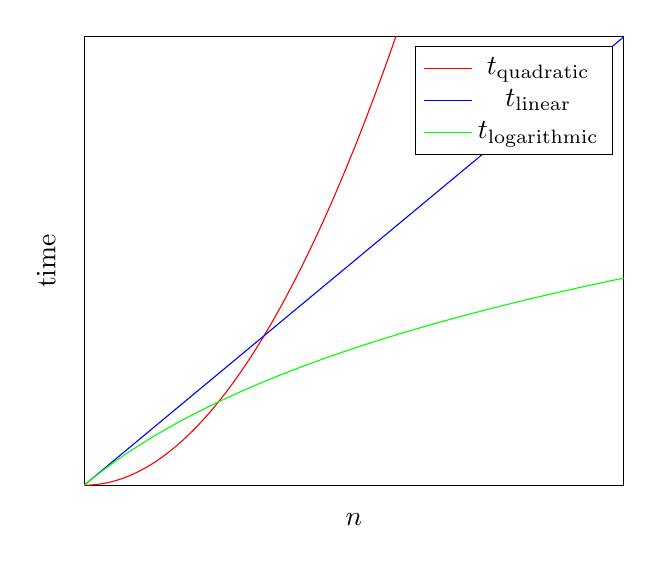
\begin{tikzpicture}
		\begin{axis}[ 
			xlabel=$n$,
			ylabel={time},
			xmin=0,
			ymin=0,
			xmax=3,
			ymax=3,
			yticklabels={,,},
			xticklabels={,,},
			tick style={draw=none}
			]
			\addplot[domain=0:3, samples=100, color=red]{x^2}; 
			\addlegendentry{\(t_{\mathrm{quadratic}}\)};
			 
			\addplot[domain=0:3, samples=100, color=blue]{x};
			\addlegendentry{\(t_{\mathrm{linear}}\)};
			
			\addplot[domain=0:3, samples=100, color=green]{ln(x+1)}; 
			\addlegendentry{\(t_{\mathrm{logarithmic}}\)};
		\end{axis}
	\end{tikzpicture}
\end{center}

We can see that logarithmic is the best scaling of the three, linear is worse, and quadratic is much worse.\\


% Course video 24
\subsection{Data Cleanup Algorithms\\ {\normalfont October 5, 2021}}
\bigbreak

The objective of these algorithms is to clean a dataset by removing undesirable items.\\

For example, you are making a survey about age. You ask 10 people ($n = 10$) and you get the following answers where 0 indicates missing data. 



\[
\renewcommand\arraystretch{1.5}
\begin{array}{|C|C|C|C|C|C|C|C|C|C|}\hline
	0 & 24 & 16 & 0 & 36 & 42 & 23 & 21 & 0 & 27 \\\hline
	\multicolumn{1}{c}{1} & \multicolumn{1}{c}{2} & \multicolumn{1}{c}{3} & \multicolumn{1}{c}{4} & \multicolumn{1}{c}{5} & \multicolumn{1}{c}{6} & \multicolumn{1}{c}{7} & \multicolumn{1}{c}{8} & \multicolumn{1}{c}{9} & \multicolumn{1}{c}{10}
\end{array}
\]\bigbreak

Let's say you want to find the average. If you take it directly, you would get that the average = $\frac{0+24+16+...+27}{10} = 18.9$ years. This is clearly not correct.\\

If instead you clean the data or account for the bad values, then you would get that the average = $\frac{24+16+...+27}{7} = 27$ years.\\

We will look at three data clean up algorithms:

\begin{itemize}
	\item The Shuffle Left
	\item The Copy-Over
	\item The Converging Pointers
\end{itemize}\bigbreak

% Course video 25, 26, 27
\subsubsection{The Shuffle Left Algorithm}
\bigbreak

The idea behind this algorithm is that it will
\begin{itemize}
	\item search the list from left to right
	\item If a zero is found, shuffle list to left
	\item It will also return the number of legitimate values in the list.
\end{itemize} 

You can imagine a school bus with students spread across the bus and the bus driver wants to get all students to move to the front end. He could start at the front of the bus and move down until he finds an empty seat. Once he finds an empty seat, he tells all students to shuffle forward. He can then look for the next empty seat, and repeat this until all the empty seats are in the back end of the bus.\\

For example, if we have the following list ($n = 6$)

\[
\renewcommand\arraystretch{1.5}
\begin{array}{|C|C|C|C|C|C|}\hline
	24 & 0 & 49 & 0 & 27 & 18 \\\hline
	\multicolumn{1}{c}{\color{green}\uparrow} & \multicolumn{1}{c}{\color{red}\uparrow} & \multicolumn{1}{c}{} & \multicolumn{1}{c}{} & \multicolumn{1}{c}{} & \multicolumn{1}{c}{}
\end{array}
\]\bigbreak

Let us define a pointer called Left (denoted in green) which indicates the index searching for zeros, and a pointer called Right (denoted in red) indicating position shuffle. We will also let Legit be the number of legit (here, non-zero) values. Initially, Left = 1, Right = 2, and Legit = $n$ = 6.\\

Now, we check if the value at position Left (green arrow) is legit, if it is, we increment Left and Right, so the list becomes:

\[
\renewcommand\arraystretch{1.5}
\begin{array}{|C|C|C|C|C|C|}\hline
	24 & 0 & 49 & 0 & 27 & 18 \\\hline
	\multicolumn{1}{c}{} & \multicolumn{1}{c}{\color{green}\uparrow} & \multicolumn{1}{c}{\color{red}\uparrow} & \multicolumn{1}{c}{} & \multicolumn{1}{c}{} & \multicolumn{1}{c}{}
\end{array}
\]\bigbreak

Now, we check if the value at position Left (green arrow) is legit, if it isn't we shuffle all values on the right of Left to the left and Legit is decremented. The list is now

\[
\renewcommand\arraystretch{1.5}
\begin{array}{|C|C|C|C|C|C|}\hline
	24 & 49 & 0 & 27 & 18 & 18 \\\hline
	\multicolumn{1}{c}{} & \multicolumn{1}{c}{\color{green}\uparrow} & \multicolumn{1}{c}{\color{red}\uparrow} & \multicolumn{1}{c}{} & \multicolumn{1}{c}{} & \multicolumn{1}{c}{}
\end{array}
\]\bigbreak

with Legit = 5. Note that the last value is duplicated. Also note that the Right pointer is used to do the shuffling. This process repeats.

\[
\renewcommand\arraystretch{1.5}
\begin{array}{|C|C|C|C|C|C|}\hline
	24 & 49 & 0 & 27 & 18 & 18 \\\hline
	\multicolumn{1}{c}{} & \multicolumn{1}{c}{} & \multicolumn{1}{c}{\color{green}\uparrow} & \multicolumn{1}{c}{\color{red}\uparrow} & \multicolumn{1}{c}{} & \multicolumn{1}{c}{}
\end{array}
\]\bigbreak

\[
\renewcommand\arraystretch{1.5}
\begin{array}{|C|C|C|C|C|C|}\hline
	24 & 49 & 27 & 18 & 18 & 18 \\\hline
	\multicolumn{1}{c}{} & \multicolumn{1}{c}{} & \multicolumn{1}{c}{\color{green}\uparrow} & \multicolumn{1}{c}{\color{red}\uparrow} & \multicolumn{1}{c}{} & \multicolumn{1}{c}{}
\end{array}
\]\bigbreak

And now Legit = 4. 

\[
\renewcommand\arraystretch{1.5}
\begin{array}{|C|C|C|C|C|C|}\hline
	24 & 49 & 27 & 18 & 18 & 18 \\\hline
	\multicolumn{1}{c}{} & \multicolumn{1}{c}{} & \multicolumn{1}{c}{} & \multicolumn{1}{c}{\color{green}\uparrow} & \multicolumn{1}{c}{\color{red}\uparrow} & \multicolumn{1}{c}{}
\end{array}
\]\bigbreak

Since Left = Legit, the algorithm halts.\\

Let's build the algorithm.

\begin{algorithm}
	\caption{Shuffle Left}
	\begin{algorithmic}[1]
		\Get $n, L_1, ..., L_n$
		\Set Legit = $n$
		\Set Left, Right = 1, 2
		\While{(Left $\le$ Legit)} step 5 to step 11
			\If{($L_{\mathrm{Left}}$ $\ne$ 0)}
				\Setx{2} Left = Left + 1
				\Setx{2} Right = Right + 1
			\Else
				\While{(Right $\leq$ Legit)} step 8 to 9
					\Set $L_{\mathrm{Right} - 1}$ = $L_{\mathrm{Right}}$
					\Set Right = Right + 1
				\EndWhile
				\Set Right = Left + 1
				\Set Legit = Legit - 1
			\EndIf
		\EndWhile
		\Stop
	\end{algorithmic}
\end{algorithm}


We will now do the complexity analysis.\\

\textbf{Best case scenario:} This occurs when there are no 0s in the list, since there are no shuffles. The number of iterations in this case is $n$. The complexity is $\Theta(n)$.\\

\textbf{Worst case scenario:} This occurs when the list entirely consists of 0s, since there are the maximum amount shuffles. The number of iterations in this case is $n - 1$ on the first shuffle, $n - 2$ on the second, etc. This means that the number of iterations is $1+2+3+...+(n-1) = \frac{n(n-1)}{2} = \frac{n^2}{2} - \frac{n}{2} \approx \frac{1}{2} n^2$. The complexity is $\Theta(n^2)$.\\


% Course video 28
\subsubsection{The Copy-Over Algorithm}
\bigbreak

The idea behind this algorithm is to scan the algorithm left to right and if a non-zero is found (legit), copy it into a new list.\\

For example, we will have the list L (size $n=8$) and we will move the legit values into the list newlist (size not yet known). We will make $i$ our pointer for iterating through L.

\[
\renewcommand\arraystretch{1.5}
\begin{array}{C|C|C|C|C|C|C|C|C|}\cline{2-9}
	L:~~~ & 23 & 0 & 45 & 42 & 0 & 0 & 2 & 7 \\\cline{2-9}
	\multicolumn{1}{c}{i} & \multicolumn{1}{c}{\uparrow} 
\end{array}
\]

\[
\renewcommand\arraystretch{1.5}
\begin{array}{C|CCCCC}\cline{2-6}
	newlist:~ & & & & & \\\cline{2-6}
\end{array}
\]\bigbreak

We can see that the first entry is non-zero, therefore, we put it into the newlist. We also increment $j$ which is a pointer for newlist.

\[
\renewcommand\arraystretch{1.5}
\begin{array}{C|C|C|C|C|C|C|C|C|}\cline{2-9}
	L:~~~ & 23 & 0 & 45 & 42 & 0 & 0 & 2 & 7 \\\cline{2-9}
	\multicolumn{1}{c}{i} & \multicolumn{1}{c}{\uparrow} 
\end{array}
\]

\[
\renewcommand\arraystretch{1.5}
\begin{array}{C|C|CCCC}\cline{2-6}
	newlist:~~~ & 23 & & & & \\\cline{2-6}
	\multicolumn{1}{c}{j} & \multicolumn{1}{c}{\uparrow}
\end{array}
\]\bigbreak

Then, we increment $i$ and repeat.

\[
\renewcommand\arraystretch{1.5}
\begin{array}{C|C|C|C|C|C|C|C|C|}\cline{2-9}
	L:~~~ & 23 & 0 & 45 & 42 & 0 & 0 & 2 & 7 \\\cline{2-9}
	\multicolumn{1}{c}{i} & \multicolumn{1}{c}{~} & \multicolumn{1}{c}{\uparrow} 
\end{array}
\]

\[
\renewcommand\arraystretch{1.5}
\begin{array}{C|C|CCCC}\cline{2-6}
	newlist:~~~ & 23 & & & & \\\cline{2-6}
	\multicolumn{1}{c}{j} & \multicolumn{1}{c}{\uparrow}
\end{array}
\]\bigbreak

Since $L_i$ is 0 here, we do not put that element in newlist (and we do not increment $j$). Instead, we simply increment $i$ and repeat.

\[
\renewcommand\arraystretch{1.5}
\begin{array}{C|C|C|C|C|C|C|C|C|}\cline{2-9}
	L:~~~ & 23 & 0 & 45 & 42 & 0 & 0 & 2 & 7 \\\cline{2-9}
	\multicolumn{1}{c}{i} & \multicolumn{1}{c}{~} & \multicolumn{1}{c}{~} & \multicolumn{1}{c}{\uparrow} 
\end{array}
\]

\[
\renewcommand\arraystretch{1.5}
\begin{array}{C|C|C|CCC}\cline{2-6}
	newlist:~~~ & 23 & 45 & & & \\\cline{2-6}
	\multicolumn{1}{c}{j} & \multicolumn{1}{c}{~} & \multicolumn{1}{c}{\uparrow}
\end{array}
\]\bigbreak

This whole process repeats until the lists and pointers look like this.

\[
\renewcommand\arraystretch{1.5}
\begin{array}{C|C|C|C|C|C|C|C|C|}\cline{2-9}
	L:~~~ & 23 & 0 & 45 & 42 & 0 & 0 & 2 & 7 \\\cline{2-9}
	\multicolumn{1}{c}{i} & \multicolumn{1}{c}{~} & \multicolumn{1}{c}{~} & \multicolumn{1}{c}{~} & \multicolumn{1}{c}{~} & \multicolumn{1}{c}{~} & \multicolumn{1}{c}{~} & \multicolumn{1}{c}{~} & \multicolumn{1}{c}{\uparrow} 
\end{array}
\]

\[
\renewcommand\arraystretch{1.5}
\begin{array}{C|C|C|C|C|C|}\cline{2-6}
	newlist:~~~ & 23 & 45 & 42 & 2 & 7 \\\cline{2-6}
	\multicolumn{1}{c}{j} & \multicolumn{1}{c}{~} & \multicolumn{1}{c}{~} & \multicolumn{1}{c}{~} & \multicolumn{1}{c}{~} & \multicolumn{1}{c}{\uparrow}
\end{array}
\]\bigbreak

\bigbreak Building the algorithm, we have


\begin{algorithm}
	\caption{Copy-Over}
	\begin{algorithmic}[1]
		\Get $n, L_1, ..., L_n$
		\Set i = 1
		\Set j = 1
		\While{(i $\le$ n)} step 5 to step 6
			\If{($L_i \ne 0$)}
				\Setx{2} $\mathrm{newlist}_j$ = $L_i$
				\Setx{2} j = j + 1
			\EndIf
			\Set i = i + 1
		\EndWhile
		\Stop
	\end{algorithmic}
\end{algorithm}\bigbreak


Now, for the complexity analysis.\\

There is no best or worse case scenarios in this algorithm. There is always $n$ iterations. That means that the \textbf{time complexity} is $\Theta(n)$.\\

Compared to the last algorithm, this is a much more efficient algorithm in time. However, the \textbf{space complexity} is worse. It requires double storage space.\\


\pagebreak
% Course video 29 and 30
\subsubsection{The Converging Pointers Algorithm}
\bigbreak

The idea behind this algorithm is that there are two pointers, Left and Right. 
\begin{itemize}
	\item Left moves up only if it is pointing at a non-zero value.
	\item If Left points at zero, copy the value at Right into Left and decrement Right by 1.
	\item Stop when Left = Right
\end{itemize}

For example, consider the following list (with $n = 8$). The blue arrow will represent the {\color{blue}Left} pointer and the red will represent the {\color{red}Right} pointer.

\[
\renewcommand\arraystretch{1.5}
\begin{array}{|C|C|C|C|C|C|C|C|}\hline
	0 & 24 & 16 & 0 & 23 & 21 & 0 & 27 \\\hline
	\multicolumn{1}{c}{\color{blue}\uparrow} & \multicolumn{1}{c}{~} & \multicolumn{1}{c}{~} & \multicolumn{1}{c}{~} & \multicolumn{1}{c}{~} & \multicolumn{1}{c}{~} & \multicolumn{1}{c}{~} & \multicolumn{1}{c}{\color{red}\uparrow}
\end{array}
\]\bigbreak

Notice that Left = 1 and Right = $n$ = 8. \\

Since the value at Left is 0, we put the value at Right into Left and decrement Right by 1. The list becomes

\[
\renewcommand\arraystretch{1.5}
\begin{array}{|C|C|C|C|C|C|C|C|}\hline
	27 & 24 & 16 & 0 & 23 & 21 & 0 & 27 \\\hline
	\multicolumn{1}{c}{\color{blue}\uparrow} & \multicolumn{1}{c}{~} & \multicolumn{1}{c}{~} & \multicolumn{1}{c}{~} & \multicolumn{1}{c}{~} & \multicolumn{1}{c}{~} & \multicolumn{1}{c}{\color{red}\uparrow} & \multicolumn{1}{c}{~}
\end{array}
\]\bigbreak

Now, Left moves forward until it is at a zero.

\[
\renewcommand\arraystretch{1.5}
\begin{array}{|C|C|C|C|C|C|C|C|}\hline
	27 & 24 & 16 & 0 & 23 & 21 & 0 & 27 \\\hline
	\multicolumn{1}{c}{~} & \multicolumn{1}{c}{~} & \multicolumn{1}{c}{~} & \multicolumn{1}{c}{\color{blue}\uparrow} & \multicolumn{1}{c}{~} & \multicolumn{1}{c}{~} & \multicolumn{1}{c}{\color{red}\uparrow} & \multicolumn{1}{c}{~}
\end{array}
\]\bigbreak

The entry at the Right pointer gets copied into the Left pointer and Right is decremented, giving

\[
\renewcommand\arraystretch{1.5}
\begin{array}{|C|C|C|C|C|C|C|C|}\hline
	27 & 24 & 16 & 0 & 23 & 21 & 0 & 27 \\\hline
	\multicolumn{1}{c}{~} & \multicolumn{1}{c}{~} & \multicolumn{1}{c}{~} & \multicolumn{1}{c}{\color{blue}\uparrow} & \multicolumn{1}{c}{~} & \multicolumn{1}{c}{\color{red}\uparrow} & \multicolumn{1}{c}{~} & \multicolumn{1}{c}{~}
\end{array}
\]\bigbreak

This process repeats until the pointers converge.

\[
\renewcommand\arraystretch{1.5}
\begin{array}{|C|C|C|C|C|C|C|C|}\hline
	27 & 24 & 16 & 21 & 23 & 21 & 0 & 27 \\\hline
	\multicolumn{1}{c}{~} & \multicolumn{1}{c}{~} & \multicolumn{1}{c}{~} & \multicolumn{1}{c}{\color{blue}\uparrow} & \multicolumn{1}{c}{\color{red}\uparrow} & \multicolumn{1}{c}{~} & \multicolumn{1}{c}{~} & \multicolumn{1}{c}{~}
\end{array}
\]\bigbreak

\[
\renewcommand\arraystretch{1.5}
\begin{array}{|C|C|C|C|C|C|C|C|}\hline
	27 & 24 & 16 & 21 & 23 & 21 & 0 & 27 \\\hline
	\multicolumn{1}{c}{~} & \multicolumn{1}{c}{~} & \multicolumn{1}{c}{~} & \multicolumn{1}{c}{~} & \multicolumn{1}{c}{{\color{blue}\uparrow}{\color{red}\uparrow}} & \multicolumn{1}{c}{~} & \multicolumn{1}{c}{~} & \multicolumn{1}{c}{~}
\end{array}
\]\bigbreak

The number of legit values is equal to the converged pointers. All of the legit values are to the left of the converged pointers. Note that this algorithm does not preserve order.\\

We can now build the algorithm.

\begin{algorithm}
	\caption{Converging Pointers}
	\begin{algorithmic}[1]
		\Get $n, L_1, ..., L_n$
		\Set Left = 1, Right = $n$
		\While{(Left $\le$ Right)} step 4 to step 5
			\If{($L_{\mathrm{Left}} \ne 0$)}
				\Setx{2} Left = Left + 1
			\Else
				\Setx{2} $L_{\mathrm{Left}}$ = $L_{\mathrm{Right}}$
				\Setx{2} Right = Right + 1
			\EndIf
		\EndWhile
		\Stop
	\end{algorithmic}
\end{algorithm}\bigbreak

We will now do the complexity analysis.\\

There is, again, no best or worse cases. The number of iterations is always $n$. Therefore, the complexity is $\Theta(n)$. 





\end{document}
